\begin{question}
\noindent A space exploration exhibit designer is enlarging a triangular logo, shape $L$, on a display grid to create a larger version, shape $L'$, using centre of enlargement $O$.

\begin{center}
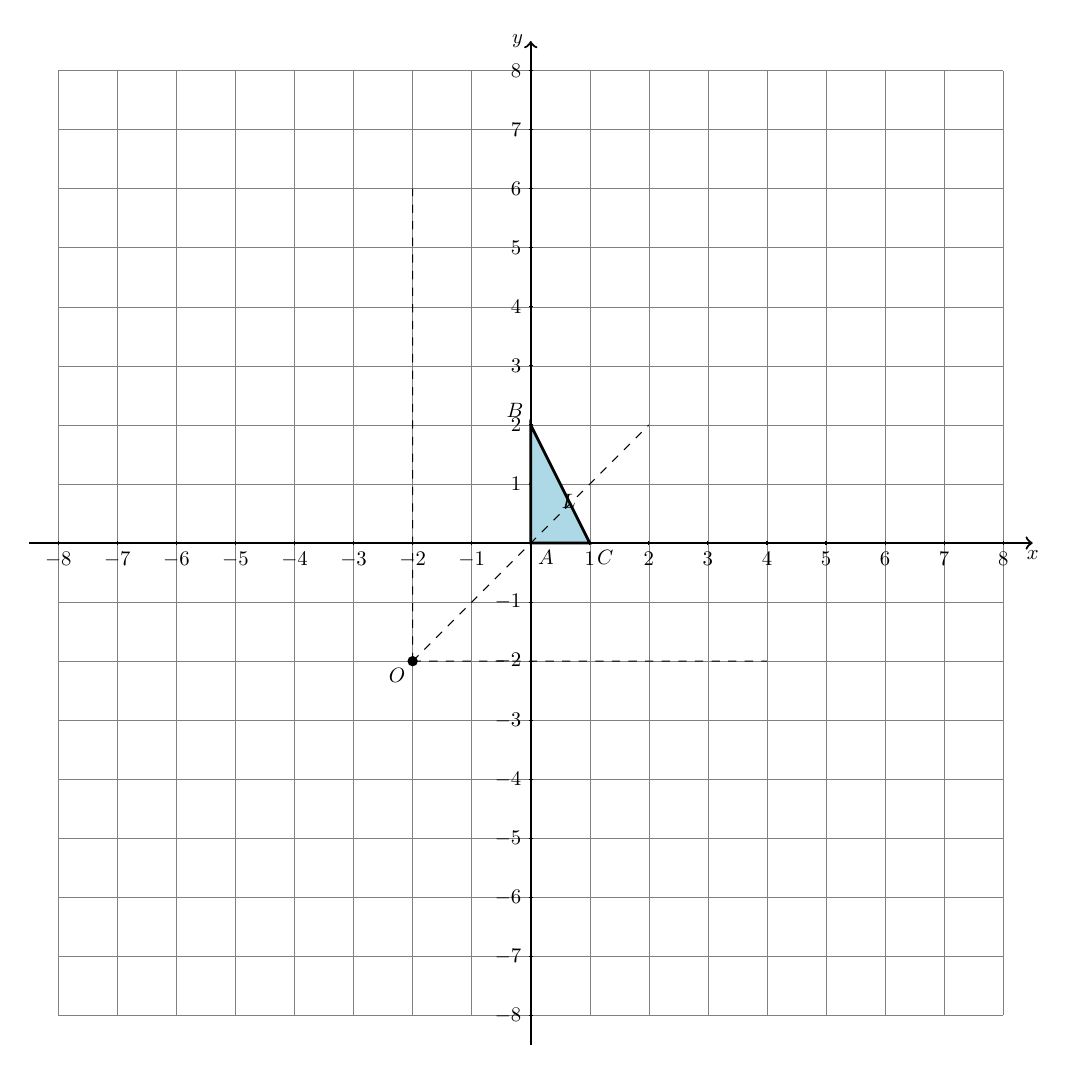
\begin{tikzpicture}[scale=0.75, transform shape]
    \definecolor{borderColour}{HTML}{000000}
    \definecolor{fillColourL}{HTML}{ADD8E6}
    \definecolor{fillColourLprime}{HTML}{D8D8D8}

    \def\axisLimit{8}

    % Draw grid
    \draw[step=1cm,gray,very thin] (-\axisLimit,-\axisLimit) grid (\axisLimit,\axisLimit);

    % Draw axes
    \draw[thick,->] (-\axisLimit-0.5,0) -- (\axisLimit+0.5,0) node[anchor=north] {$x$};
    \draw[thick,->] (0,-\axisLimit-0.5) -- (0,\axisLimit+0.5) node[anchor=east] {$y$};

    % Label x-axis and y-axis
    \foreach \x in {-\axisLimit,...,-1,1,2,...,\axisLimit}
        \draw (\x cm,1pt) -- (\x cm,-1pt) node[anchor=north] {$\x$};
    \foreach \y in {-\axisLimit,...,-1,1,2,...,\axisLimit}
        \draw (1pt,\y cm) -- (-1pt,\y cm) node[anchor=east] {$\y$};

    % Centre of enlargement O at (-2,-2)
    \coordinate (O) at (-2,-2);
    \fill[black] (O) circle (2.5pt);
    \node[below left] at (O) {$O$};

    % Shape L: A(0,0), B(0,2), C(1,0)
    \coordinate (A) at (0,0);
    \coordinate (B) at (0,2);
    \coordinate (C) at (1,0);
    \filldraw[fill=fillColourL, draw=borderColour, line width=1pt] (A) -- (B) -- (C) -- cycle;
    \node[right] at (0.4,0.7) {$L$};

    \node[below right] at (A) {$A$};
    \node[above left] at (B) {$B$};
    \node[below right] at (C) {$C$};

    % Draw construction rays from O through A, B, C extended to images
    \draw[dashed] (O) -- (2,2);
    \draw[dashed] (O) -- (-2,6);
    \draw[dashed] (O) -- (4,-2);

\end{tikzpicture}
\end{center}

\noindent On the grid, $O$ is the centre of enlargement at $(-2,-2)$, and triangle $L$ has vertices $A(0,0)$, $B(0,2)$ and $C(1,0)$.

\noindent Enlarge triangle $L$ by scale factor $2$, using $O$ as the centre of enlargement. Label the image $L'$.

\vspace{4cm}

\begin{flushright}
    \answerplain{3}
\end{flushright}
\end{question}
